% Created 2021-01-21
% Intended LaTeX compiler: pdflatex
\documentclass[11pt]{article}
\usepackage[utf8]{inputenc}
\usepackage[T1]{fontenc}
\usepackage{graphicx}
\usepackage{grffile}
\usepackage{longtable}
\usepackage{wrapfig}
\usepackage{rotating}
\usepackage[normalem]{ulem}
\usepackage{amsmath}
\usepackage{textcomp}
\usepackage{amssymb}
\usepackage{capt-of}
\usepackage{hyperref}
\usepackage{algorithm}
\usepackage[noend]{algpseudocode}
\usepackage{algorithmicx}
\author{Mingzhe Wang\\wangm235@mcmaster.ca
\and Xing Li\\li64@mcmaster.ca}
\date{\today}
\title{Assignment 1}

% algpseudocode modifications
\newcommand*{\Let}[2]{\State #1 $\gets$ \parbox[t]{\linegoal}{#2\strut}}
\algnewcommand\algorithmicinput{\textbf{INPUT: }}
\algnewcommand\Input{\item[\algorithmicinput]}
\algnewcommand\algorithmicoutput{\textbf{OUTPUT: }}
\algnewcommand\Output{\item[\algorithmicoutput]}

% algorithmic modifications
\makeatletter
\newcommand{\ALOOP}[1]{\ALC@it\algorithmicloop\ #1%
  \begin{ALC@loop}}
\newcommand{\ENDALOOP}{\end{ALC@loop}\ALC@it\algorithmicendloop}
\renewcommand{\algorithmicrequire}{\textbf{Input:}}
\renewcommand{\algorithmicensure}{\textbf{Output:}}
\newcommand{\algorithmicbreak}{\textbf{break}}
\newcommand{\BREAK}{\STATE \algorithmicbreak}
\makeatother

\begin{document}
\maketitle
\tableofcontents

\newpage
\section{Question 1}
\label{q1}
\subsection{Question1 1a}
\label{q1a}
\begin{algorithm}
\caption{Reverse Algorithm}
\begin{algorithmic}[1]
\Procedure{Reverse}{$L$}
\State $x = NIL$
\State $curr = L.head$
\While{$curr != NIL$}
\State $next = curr.next$
\State $curr.next = x$
\State $curr.prev = NIL$
\If{$x != NIL$}
\State $x.prev = curr$
\EndIf
\State $x = curr$
\State $curr = next$
\EndWhile
\State \Return x
\EndProcedure
\end{algorithmic}
\end{algorithm}

\subsection{Question1 1b}
\label{q1b}
\textbf{Explanation}: this algorithm return a new reversed list by the following step:
\begin{itemize}
\item Create a $x$ pointing to $NIL$ representing the output list and a $curr$ pointing to the original list's head.
\item The $curr$ traverse the original list and at each time lets the current node be attached to the output list by updating its $prev$ and $next$ field and the output list's $prev$ field.
\item When all the node are attached to the new list, the output list will automatically be the reversed version of the original list.
\end{itemize}
\textbf{Running time analysis}: The running time of this algorithm is $O(n)$, because the inner loop will traverse the whole original list with length $n$ only once.

\newpage
\section{Question 2}
\label{q2}
\begin{algorithm}
\caption{NSV Algorithm}
\begin{algorithmic}[1]
\Procedure{NSV}{$A$}
	\For{$i = 1$ to $A.length$}
		\State $NSV[i] = 0$
	\EndFor
	\For{$i = 1$ to $A.length$}
		\While{$!S.IsEmpty$}
			\State $j = S.pop$
			\If{$A[i] < A[j]$}
				\State $NSV[j] = i - j$
			\Else
				\State $S.push(j)$
				\State \algorithmicbreak
			\EndIf
		\EndWhile
		\If{$A[i] != 0$}
			\State $S.push(i)$
		\EndIf
	\EndFor
	\While{$!S.IsEmpty$}
		\State $i = S.pop$
		\State $NSV[i] = A.length + 1 - j$
	\EndWhile
	\State \Return $NSV$
\EndProcedure
\end{algorithmic}
\end{algorithm}

\newpage
\section{Question 3}
\label{q3}
\begin{algorithm}
\caption{Queue Using Stack}

\begin{algorithmic}[1]
\Procedure{Enqueue}{$S, x$}
	\State $S.push(x)$
\EndProcedure
\end{algorithmic}
\begin{algorithmic}[1]
\Procedure{Dequeue}{$S$}
	\If{$S.IsEmpty$}
	\State $\textbf{Error}$ $underflow$
	\EndIf
	\While{$!S.IsEmpty$}
		\State $S2.push(S.pop)$
	\EndWhile
	\State $x = S2.pop$
	\While{$!S2.IsEmpty$}
		\State $S.push(S2.pop)$
	\EndWhile
	\State \Return $x$
\EndProcedure
\end{algorithmic}
\end{algorithm}

\section{Question 4}
\label{q4}
\subsection{Question 4a}
\label{q4a}
Note: the $\Theta(n^4)$ in this problem should be $O(n^4)$.\\\\
Choose $c = 70, n_0 = 1$, we have $(65n^4 + 2n + 3) / (n^4 + 1) \leq 65n^4 + 2n + 3 \leq 70n^4$ for all $n \geq 1$. Therefore, $(65n^4 + 2n + 3) / (n^4 + 1) = O(n^4)$ holds.


\subsection{Question 4b}
\label{q4b}
$LHS = n^2 + n^2 + 1 = 2n^2 + 1$.
Choose $c_1 = 2, c_2 = 3, n_0 = 1$, we have $2n^2 \leq 2n^2 + 1 \leq 3n^2$ for all $n \geq 1$. Therefore, $\log 2^{n^2} + n^2 + 1 = \Theta(n^2)$ holds.

\subsection{Question 4c}
\label{q4c}
$LHS = \frac{(1+n)n}{2} = \frac{1}{2}n^2 + \frac{1}{2}n$.
Choose $c = 1, n_0 = 1$, we have $\frac{1}{2}n^2 + \frac{1}{2}n \leq n^2$ for any $n \geq 1$.
Therefore, $1 + 2 + 3 + \ldots + n = O(n^2)$ holds.

\section{Question 5}
\label{q5}
\subsection{Question 5a}
\label{q5a}
We will prove this by contradiction. If $(1000n^4 + n^2 + 4n)/(\log n) = \Theta(n^4)$ holds, there exists $c_1, c_2, n_0$ such that $c_1 n^4 \leq (1000n^4 + n^2 + 4n)/(\log n) \leq c_2 n^4$ for all $n \geq n_0$. We will prove there is not a $c_1$ such that $c_1 n^4 \leq (1000n^4 + n^2 + 4n)/(\log n)$, (i.e. $c_1 n^4 \log n \leq 1000n^4 + n^2 + 4n$) for all $n \geq n_0$.\\\\
For any $n \geq 2^{1006 / c_1}$, $c_1 n^4 \log n > 1000n^4 + n^2 + 4n$, which is contradict to the assumption. Therefore, $(1000n^4 + n^2 + 4n)/(\log n) = \Theta(n^4)$ is false.


\subsection{Question 5c}
\label{q5c}
We will prove this by contradiction. If $\sqrt{n} = O(\log n)$ holds, there exists $c, n_0$ such that $\sqrt{n} \leq c \log n$ for all $n \geq n_0$. The inequality can be written as $\sqrt{n} \leq 2c \log \sqrt{n}$. Then there exists $c_1 = 2c, n_1 = \sqrt{n_0}$ such that $n \leq c_1 \log n$ for all $n \geq n_1$. That means $n = O(\log n)$, which is contradict to the fact $\log n = O(n)$. Therefore, $\sqrt{n} = O(\log n)$ is false.


\section{Question 6}
\label{q6}
\begin{algorithm}
\caption{Simple Algorithm}
\begin{algorithmic}[1]
\Procedure{SimpleProcedure}{}
\State $MSum \gets 0, LI \gets 0, UI \gets 0$
\For{$i = 1$ to n} // i is the length of each subset
    \For{$j = 1$ to $n+1-i$} // j is the start index of each subset of length i
        \State $Sum \gets 0$
        \For{$k = j$ to $j+i-1$} // k is the index of each element of the subset
            \State $Sum\gets Sum+x_k$
        \EndFor
        \If{$Sum \ge MSum$}
            \State $MSum \gets Sum$
            \State $LI \gets j$
            \State $UI \gets j+i-1$
        \EndIf
    \EndFor
\EndFor
\State \Return $MSum, LI, UI$
\EndProcedure
\end{algorithmic}
\end{algorithm}
\newpage
\begin{algorithm}
\caption{Better Algorithm}
\begin{algorithmic}[1]
\Procedure{BetterProcedure}{}
\State $MSum \gets 0, LI \gets 0, UI \gets 0$
\For{$i = 1$ to n} // i is the start index of each subset
    \State $Sum \gets 0$
    \For{$j = i$ to $n$} // j is the end index of each subset
        \State $Sum\gets Sum+x_j$
        \If{$Sum \ge MSum$}
            \State $MSum \gets Sum$
            \State $LI \gets i$
            \State $UI \gets j$
        \EndIf
    \EndFor
\EndFor
\State \Return $MSum, LI, UI$
\EndProcedure
\end{algorithmic}
\end{algorithm}

\section{Question 7}
\label{q7}
\begin{algorithm}
\caption{Algorithm of Comparing four numbers}
\begin{algorithmic}[1]
\Procedure{ComparingTwoNumbers}{Num1, Num2}
\State //Compare two numbers via one comparison
\If{Num1 > Num2}
    \State  $Array[0] \gets Num2, Array[1] \gets Num1$
\Else
    \State  $Array[0] \gets Num1, Array[1] \gets Num2$
\EndIf
\State \Return Array
\EndProcedure
\Procedure{ComparingFourNumbers}{Num1, Num2, Num3, Num4}
\State //Generate two arrays via two comparisons
\State $Array1 \gets ComparingTwoNumbers(Num1, Num2)$
\State $Array2 \gets ComparingTwoNumbers(Num3, Num4)$
\State //Merge the two arrays via at most three comparisons
\If{Array1[0] > Array2[0]}
    \State $FinalArray[0] \gets Array2[0]$
    \If{Array1[0] > Array2[1]}
        \State $FinalArray[1] \gets Array2[1]$,$FinalArray[2] \gets Array1[0]$,$FinalArray[3] \gets Array1[1]$
    \Else
        \State $FinalArray[1] \gets Array1[0]$
        \If{Array1[1] > Array2[1]}
            \State $FinalArray[2] \gets Array2[1], FinalArray[3] \gets Array1[1]$
        \Else
            \State $FinalArray[2] \gets Array1[1], FinalArray[3] \gets Array2[1]$            
        \EndIf
    \EndIf
\Else
    \State $FinalArray[0] \gets Array1[0]$
    \If{Array1[1] > Array2[0]}
        \State $FinalArray[1] \gets Array2[0]$
        \If{Array1[1] > Array2[1]}
            \State $FinalArray[2] \gets Array2[1], FinalArray[3] \gets Array1[1]$
        \Else
            \State $FinalArray[2] \gets Array1[1], FinalArray[3] \gets Array2[1]$            
        \EndIf
    \Else
        \State $FinalArray[1] \gets Array1[1]$, $FinalArray[2] \gets Array2[0]$, $FinalArray[3] \gets Array2[1]$
    \EndIf
\EndIf
\State \Return FinalArray
\EndProcedure
\end{algorithmic}
\end{algorithm}

\newpage
\section{Question 8}
\label{q8}
\begin{center}
\begin{tabular}{ c|c|c|c|c|c|c|c|c|c|c }
9 & 1 & 5 & 2 & 11 & 18 & 7 & 23 & 13 & 0 & 4
\end{tabular}
\\Split\\
\begin{tabular}{ c|c|c|c|c|c|c|c|c|c|c|c } 
9 & 1 & 5 & 2 & 11 & \ + \ &18 & 7 & 23 & 13 & 0 & 4
\end{tabular}
\\Split\\
\begin{tabular}{ c|c|c|c|c|c|c|c|c|c|c|c|c|c } 
9 & 1 &\ + \ & 5 & 2 & 11 & \ + \ &18 & 7 & 23 &\ +\ & 13 & 0 & 4
\end{tabular}
\\Split\\
\begin{tabular}{ c|c|c|c|c|c|c|c|c|c|c|c|c|c|c|c|c } 
9 & 1 &\ + \ & 5 & \ + \ & 2 & 11 & \ + \ &18 & \ + \ & 7 & 23 &\ +\ & 13& \ + \ &  0 & 4
\end{tabular}
\\Sort\\
\begin{tabular}{ c|c|c|c|c|c|c|c|c|c|c|c|c|c|c|c|c } 
1 & 9 &\ + \ (& 5 & \ + \ & 2 & 11 &) \ + \ (&18 & \ + \ & 7 & 23 &)\ +\ (& 13& \ + \ &  0 & 4)
\end{tabular}
\\Merge\\
\begin{tabular}{ c|c|c|c|c|c|c|c|c|c|c|c|c|c } 
(1 & 9 &\ + \ & 2 & 5 & 11 &) \ + \ (&7 & 18 & 23 &\ +\ & 0 & 4 & 13)
\end{tabular}
\\Merge\\
\begin{tabular}{ c|c|c|c|c|c|c|c|c|c|c|c } 
1 & 2 & 5 & 9 & 11 & \ + \ &0 & 4 & 7 & 13 & 18 & 23
\end{tabular}
\\Merge\\
\begin{tabular}{ c|c|c|c|c|c|c|c|c|c|c|c } 
0 & 1 & 2 & 4 & 5 &7 & 9 & 11 & 13 & 18 & 23
\end{tabular}
\end{center}

\newpage
\section{Question 9}
\label{q9}
\begin{algorithm}
\caption{Algorithm of Quicksort without Recursion}
\begin{algorithmic}[1]
\Procedure{QuickSort}{S}
\State Push {S}
\State $Result \gets empty\ list $
\While{Stack is not empty}
    \State $S \gets Pop$
    \If{$|S| \le 3$}
        \State InsertionSort S
        \State Concatenate(Result, S)
    \Else
        \State Shuffle S
        \State Randomly pick $a_i \in S$
        \For {all $a_j \in S, j \neq i$}
            \If {$a_j \le a_i $}
                \State Put $a_j$ in $S^-$
            \Else
                \State Put $a_j$ in $S^+$
            \EndIf
        \EndFor
        \State Push $S^+$
        \State Push $a_i$
        \State Push $S^-$
    \EndIf
\EndWhile
\State \Return Result
\EndProcedure
\end{algorithmic}
\end{algorithm}
\newpage
\section{Question 10}
\label{q10}
\subsection{Question 10a}
In a max-oriented heap, the value in each internal node is greater than or equal to the values in the children of that node. An array that is sorted in decreasing order can always guarantee this. 

~\newline\noindent Suppose a heap is structured as an array a with start index 1. The index of any internal node i and the indexes of its children ($i_1$ and $i_2$) follows a rule: $i_1 = 2 * i$ and $i_2 = 2 * i + 1$ a heap is a complete binary tree.

~\newline\noindent As long as the array is sorted in decreasing order, a[i] is always greater or equal to $a[2 * i + 1]$ or $a[2 * i + 2]$. In another word, the value in each internal node is greater than or equal to the values in the children of that node.

\subsection{Question 10b}
In the discussion below, we explain with a max-oriented heap, which can be symmetrically applied to a min-oriented heap. 

~\newline\noindent 
\textbf{Heap sort using the most number of compares.}

~\newline\noindent Since the heap sort algorithm introduced in the class follows two steps: "bottom-up sink" and "remove the maximum", we can create an array requiring the most comparison in the way illustrated below.

\begin{enumerate}
\item The elements of each upper level of the heap tree are less than the lower level. This means that all elements with index $\le$ 8 needs to sink the most, and sinking the most is equivalent to comparing the most.

\item Because N = 16, and the 16th element is the ultra left element at the 4th level, we can organize the elements such that at each level, the left element is greater than the right element. Thus, the longest path is always occupied by the greatest element, which helps us sink the most.
\end{enumerate}

~\newline\noindent With the two approaches above, the array requiring the most comparison can be constructed as below.
 \begin{figure}[hbt!]
  \centering
    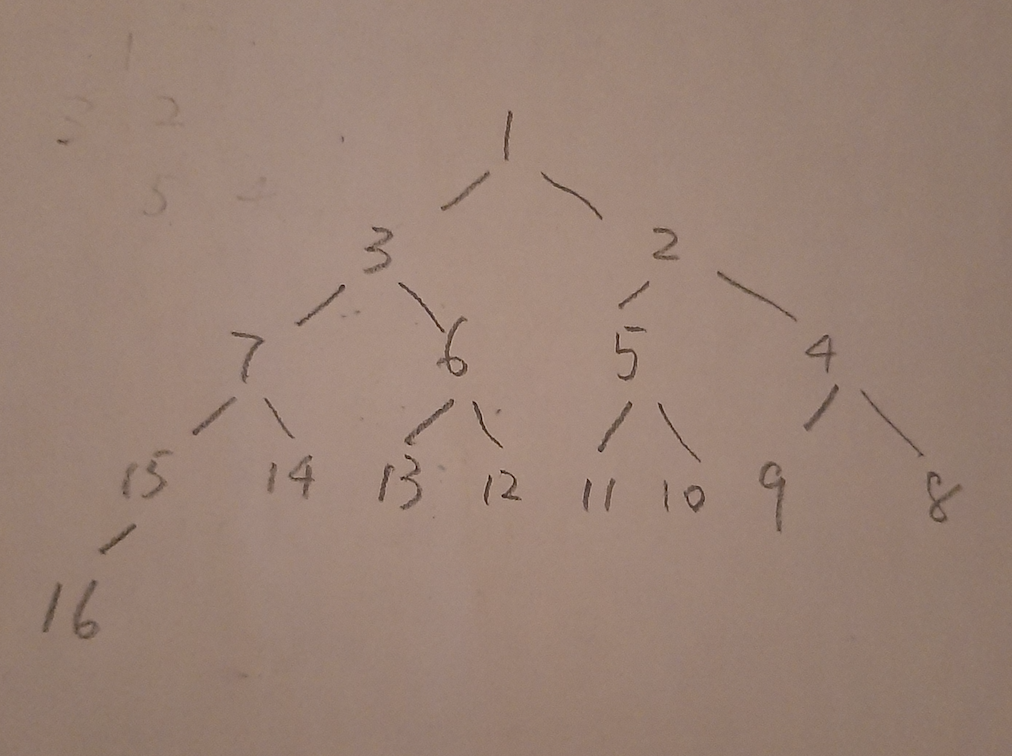
\includegraphics[width=1\textwidth]{Figures/heap.jpg}\label{heap}
  \caption{heapsort using the most number of compares}
\end{figure}
\newpage

~\newline\noindent The corresponding array is [1, 3, 2, 7, 6, 5, 4, 15, 14, 13, 12, 11, 10, 9, 8, 16].

~\newline\noindent Although this approach minimizes the comparison in the "bottom-up sink" step, we cannot guarantee minimum comparison in the  "remove the maximum" step. 

~\newline\noindent 
\textbf{Heap sort using the least number of compares.}

~\newline\noindent If we use the same approach, we can find a symmetric construction as shown below.

\begin{enumerate}
\item The elements of each upper level of the heap tree are greater than the lower level. This means that all elements with index $\le$ 8 needs to sink the least, and sinking the least is equivalent to comparing the least.

\item Because N = 16, and the 16th element is the ultra left element at the 4th level, we can organize the elements such that at each level, the left element is less than the right element. Thus, the longest path is always occupied by the least element, which helps us sink the least.
\end{enumerate}

~\newline\noindent The corresponding array is also symmetric: [16, 14, 15, 10, 11, 12, 13, 2, 3, 4, 5, 6, 7, 8, 9, 1].

\end{document}
